\documentclass[11pt]{article}
\usepackage[margin=0.9in]{geometry}
\usepackage{amsmath,amssymb,graphicx,booktabs,hyperref,xcolor,float}
\usepackage[T1]{fontenc}
\graphicspath{{../v3/}{../cocoa/analysis/}}
\newcommand{\hmpc}{\,h\,\mathrm{Mpc}^{-1}}
\newcommand{\dchi}{\Delta\chi^2}
\title{The Roman test on stitched FLAMINGO truths\\[2pt]\large Control variants for the k\_max analysis (supplement to the 7 Nov summary)}
\author{Yijie Zhu, with Claude}
\date{7 November 2026}

\begin{document}
\maketitle

\section*{Question and answer}

The FLAMINGO notes build the IA spectra as a stitch: a per-snapshot NLA fit
on large scales and the simulation on small scales, joined by a logistic
weight at a transition scale $k_t(z)$. The question was whether running the
Roman test on that stitched truth instead of the production
(spline-smoothed, simulation-only) truth would help. This supplement runs
it, with three related variants, through the same all-parameters-free fit
as Section 8 of the main summary. The result is more informative than
expected, because the stitch separates two failure modes that the
production truth mixes.

\begin{itemize}
\item \textbf{The FoB is lower on every mask, but less than the construction
  suggests.} With the B-plateau $N_s$ (variant S1) the FoB = 0.3 crossing
  in the $K_0/D(z)$ family moves from $K_0 \approx 0.30$ to $\approx 0.34$
  (NLA) and $\approx 0.39$ (TATT). With the notes' $N_s$ (S2, S3) NLA stays
  at or below 0.28 up to $K_0 = 0.5$ and TATT crosses near 0.45. On the flat
  $z$-dependent cuts every stitched variant stays below 0.27 up to twice the
  TATT GoF cut.
\item \textbf{The misfit hardly changes.} At $K_0 = 0.3$ the best-fit
  $\chi^2$ is 1.11 / 1.05 (NLA / TATT) for S1 against 1.18 / 0.96 for the
  production truth. Nearly all of the residual misfit lives above $k_t$,
  in the simulation side that the stitch keeps.
\item \textbf{What changes is the direction of the shift.} The production
  truth biases $S_8$ (+0.3 to +0.6$\sigma$, growing with $K_0$); the stitched
  truth biases $\Omega_m$ ($-0.3\sigma$, $S_8$ within $\pm 0.1\sigma$) and the
  shift saturates for $K_0 \ge 0.35$. The $S_8$ shift is the white II excess
  (constant in $k$, enters $\xi_-$ as $\theta^{-2}$, not removable by a $k$
  mask), which the notes' NLA+$N_s$ fit absorbs into $N_s$; the $\Omega_m$
  shift is the GI/II misfit in the transition regime $0.2 \lesssim k
  \lesssim 1\hmpc$, and it is there even when the large scales are NLA by
  construction.
\item \textbf{The stitch is not conservative below $k_t$.} The notes'
  $k_t$ (0.16 to 0.27$\hmpc$ across the core snapshots) lies 1.5 to 2 times
  above the $k_{\max}$ at which the simulation rejects NLA at $p<0.05$ with
  $N_s$ fixed (0.09 to 0.12$\hmpc$), and 83 (90) per cent of the Roman
  $\xi_\pm$ weight sits at $k \le 0.16$ (0.22)$\hmpc$. The stitch therefore
  replaces a measured departure from NLA by NLA over the band that decides
  the cut.
\item \textbf{S4} (production above the data $k_{\min} = 0.05$, NLA below,
  hard join) raises $\chi^2$ by 0.3 to 1.0 and moves the FoB by at most
  0.05; the change is the kink at 0.05 in the white term. The smooth
  version of this variant (white term kept white below 0.05,
  \texttt{bias\_phys.py} in the main summary) changes the FoB by less than
  0.02. The low-$k$ extrapolation is worth one sentence in the paper, not
  more.
\item \textbf{Recommendation.} Keep the production truth for the Part 2
  numbers. Report the stitched result as the control it is: ``even if the
  IA is assumed to be NLA below $k_t(z)$, the transition-regime misfit
  alone shifts $\Omega_m$ by $0.3\sigma$ at $K_0 \approx 0.34$ (NLA) /
  0.39 (TATT)''. And make the white II term an explicit decision in the
  paper (keep it, or remove it with the one-parameter template of the
  main summary), because it decides whether the bias appears in $S_8$ or
  in $\Omega_m$.
\end{itemize}

\section{Truth variants}

All variants are ratios $R_X(k, z) = P_X / P_{\rm NL}$ per snapshot on the
26-point combined-fold grid ($0.009 \le k \le 17.7\hmpc$), converted to
sim\_IA tables on the wide grid exactly as the production truth (linear in
$\ln k$, edge values held outside), so that truth and models share the Limber
integration, the $C_\ell \to \xi_\pm$ transform and the bin averaging. The
rebuilt production tables reproduce the stored production $\xi_{\rm FL}$ to
machine precision.

\paragraph{Production (``prod'').} Weighted smoothing spline of the measured
ratios on $k \ge 0.05$ ($\chi^2 = N$), ratio held at its $k = 0.05$ value
below, $P_{EE}$ minus the white shape noise $N_s^{B}$ (median $P_{BB}$ of the
nfold-4 data at $5 < k < 10\hmpc$).

\paragraph{Stitch (notes' recipe).} With $w(k) = \left[1 + \exp\!\left(-\ln(k/k_t)/\sigma_w\right)\right]^{-1}$,
$\sigma_w = 0.30$, and $(-C_1, C_1^2)$ the NLA fit (with a free $N_s$) to the
nfold-1 data on $0.05 \le k \le 0.3$,
\begin{align}
R_{\delta E} &= -(1-w)\,C_1 + w\,\frac{P_{hE}}{b(k)\,P_{\rm NL}}, \\
R_{EE} &= (1-w)\,C_1^2 + w\,\frac{P_{EE} - N_s}{P_{\rm NL}} .
\end{align}
\begin{itemize}
\item \textbf{S1}: simulation side = the production spline, $N_s = N_s^{B}$.
  Isolates the NLA replacement from everything else.
\item \textbf{S2}: as S1 with the notes' $N_s$ from the NLA+$N_s$ fit
  ($N_s^{\rm NLA}/N_s^{B}$ = 3.8, 3.6, 3.3, 2.9, 2.9, 2.7, 2.5, 2.4, 2.2, 2.1, 2.3 for
  $z$ = 0 to 2). This over-subtracts the white level above $k_t$.
\item \textbf{S3}: the notes' recipe literally (\texttt{build\_spectra.py}
  \texttt{truth\_nla}): measured simulation side, notes' $N_s$.
\item \textbf{S4}: production above $k = 0.05$, pure NLA $(-C_1, C_1^2)$ below
  the data $k_{\min}$ instead of the held ratio.
\end{itemize}
The transition scales from the notes are $k_t$ = 0.155, 0.159, 0.162, 0.167,
0.172, 0.181, 0.190, 0.200, 0.210, 0.230, 0.269, 0.345, 0.447$\hmpc$ for
$z$ = 0, 0.1, 0.2, 0.3, 0.4, 0.5, 0.6, 0.75, 1, 1.5, 2, 3, 4. For the FoB
uncertainty from the simulation's error bars (the $J_{\rm cells}\,\sigma$
propagation of Section 2 of the main summary) the simulation-side errors
are multiplied by $w(k)$ for S1 to S3.

\begin{figure}[H]
\centering
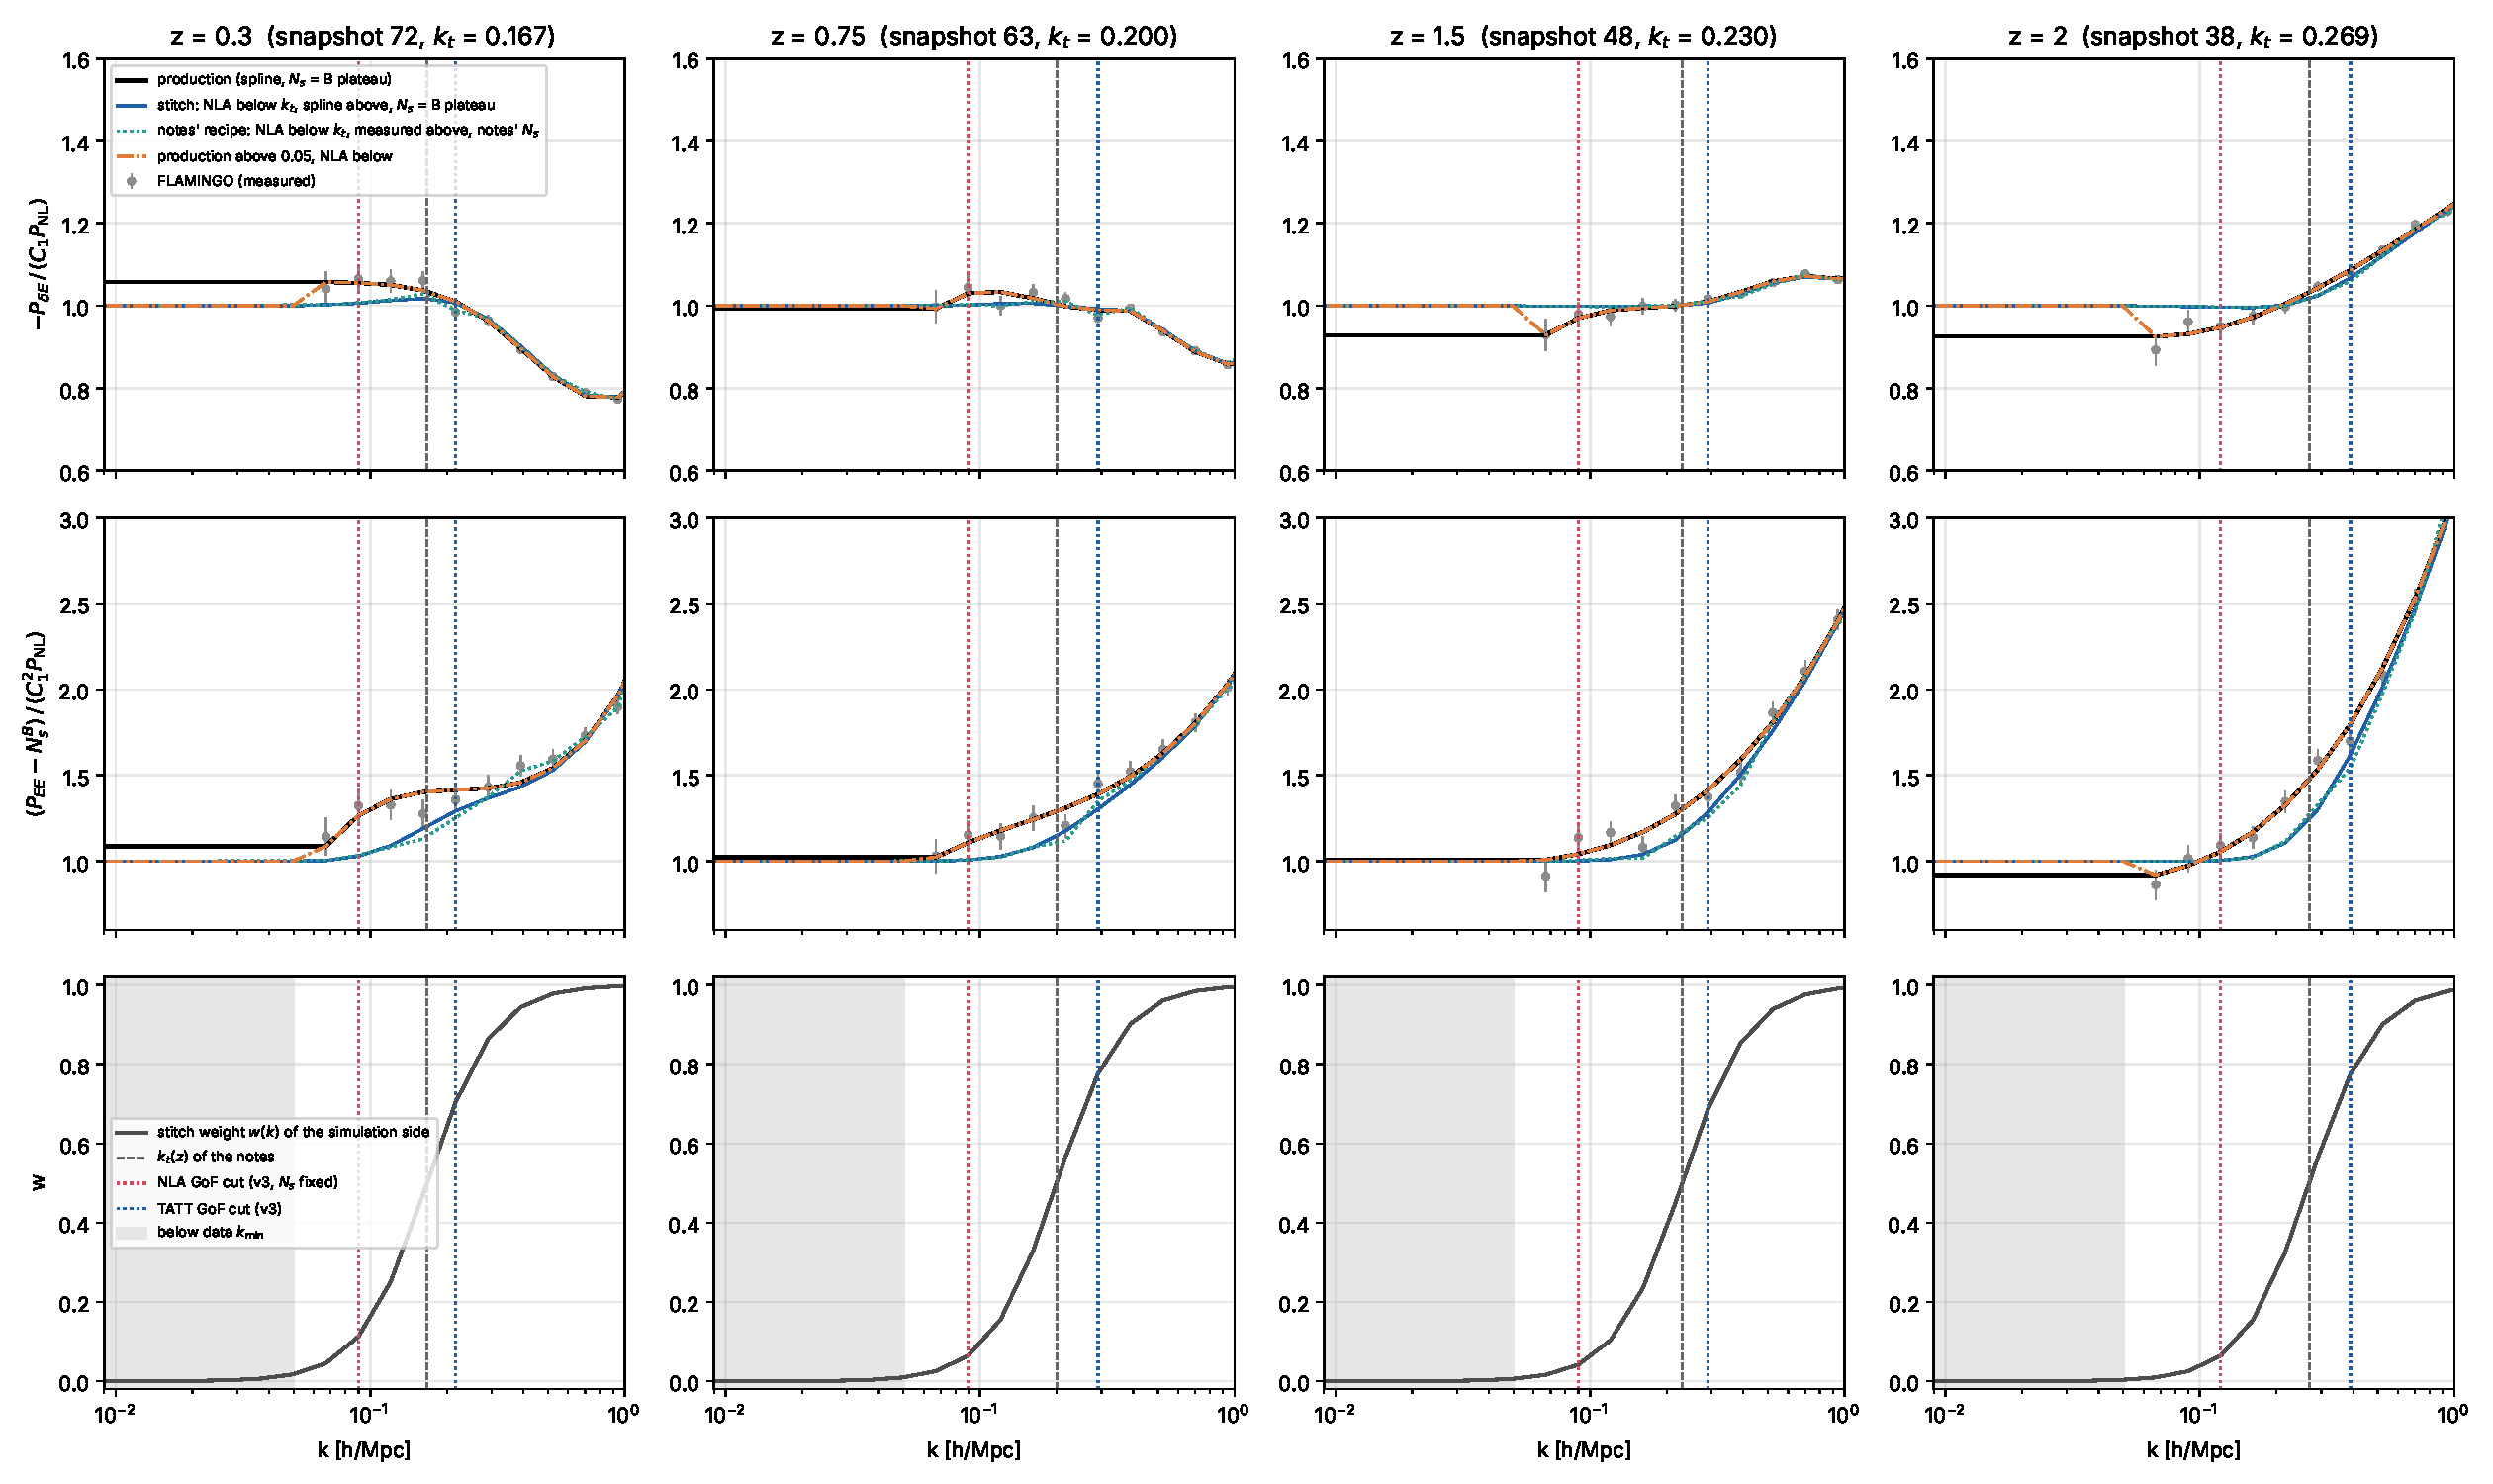
\includegraphics[width=\textwidth]{fig_stitch_truths}
\caption{The truth variants against the measured FLAMINGO ratios (grey
points with the simulation's error bars), normalised to the notes' NLA side
$(C_1, C_1^2)$, for four core snapshots. Top: GI; middle: II with the
B-plateau $N_s$ subtracted (S3 is shown on the same axis by adding back its
extra $N_s$ offset, weighted by $w$). Bottom: the stitch weight $w(k)$, the
notes' $k_t$ (grey dashed), and the $k_{\max}$ at which the v3 goodness of
fit rejects NLA (red dotted) and TATT (blue dotted) at $p<0.05$ with $N_s$
fixed. Between the red line and $k_t$ the stitched truth replaces a measured
departure from NLA by NLA.}
\end{figure}

\section{Results}

Same fit as Section 8 of the main summary: data = GG + truth variant, model =
native NLA or TATT with power-law redshift evolution, cosmology free (case A:
$\Omega_m, A_s$; case B adds $n_s, H_0, \Omega_b$ with Gaussian priors of the
chain's flat-prior width), IA bounded to the chain priors, several starts,
FoB $= \sqrt{\delta\theta^T \Sigma^{-1} \delta\theta}$ in $(\Omega_m, S_8)$
with the IA marginalised at the flat-prior width, Gaussian covariance. Masks:
the production $K_0/D(z)$ family and the flat $z$-dependent TATT-shaped cuts
$\times\{1, 1.4, 2\}$.

\begin{figure}[H]
\centering
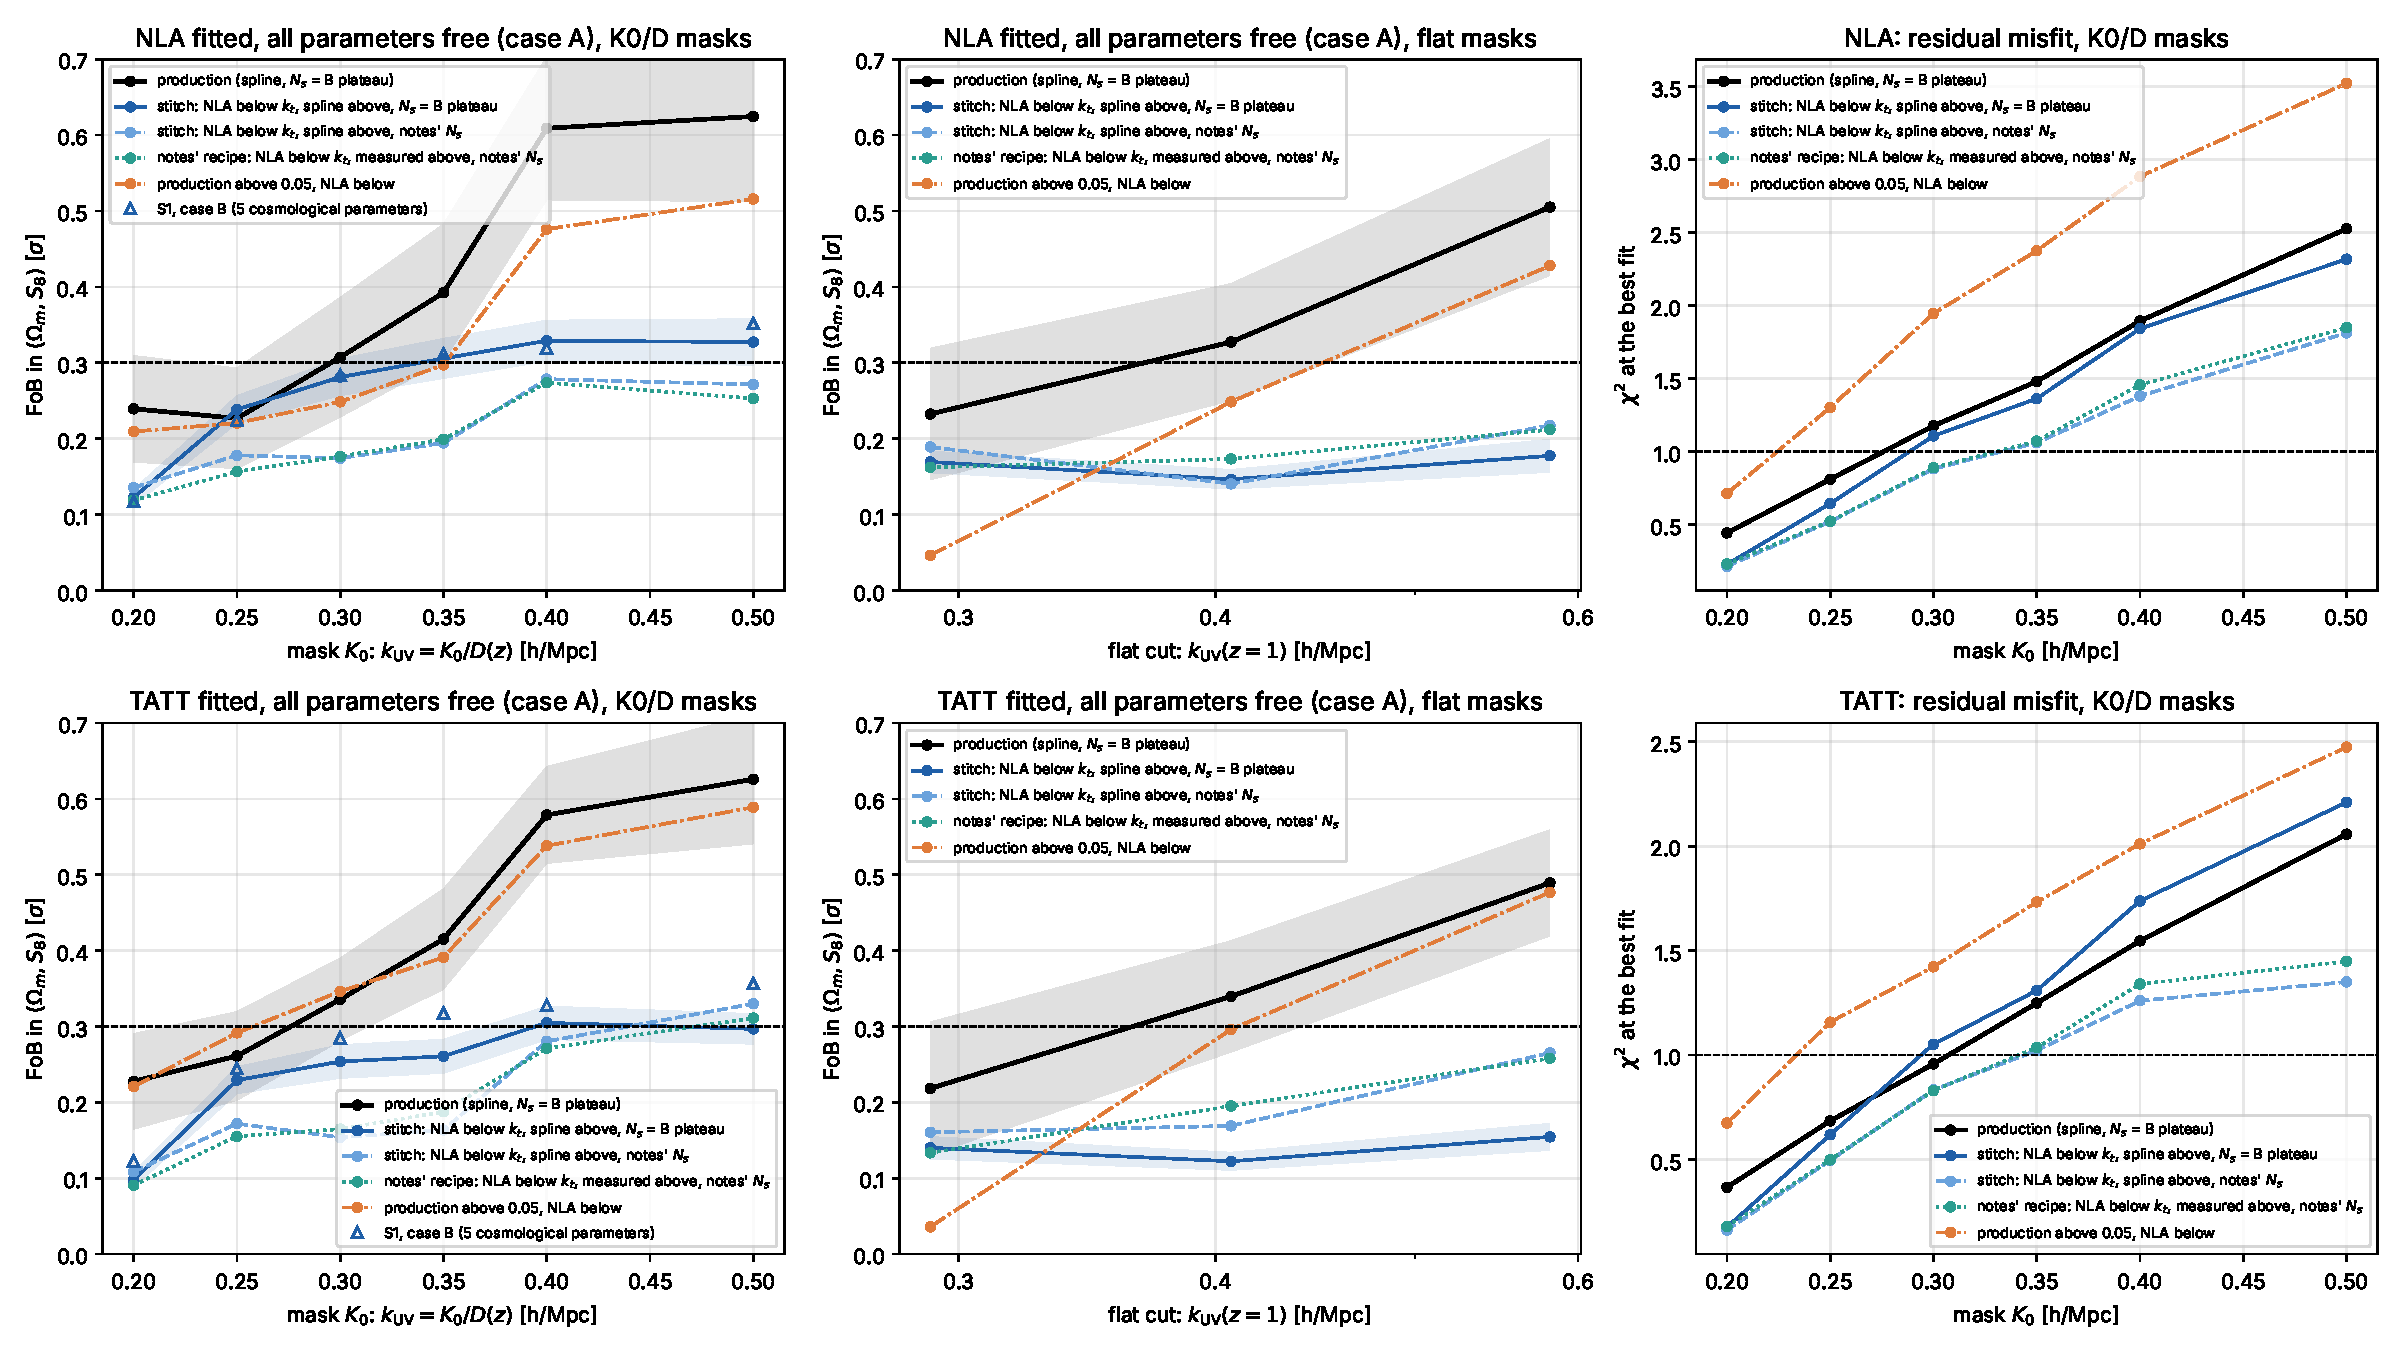
\includegraphics[width=\textwidth]{fig_stitch_fob}
\caption{FoB (left, middle) and best-fit $\chi^2$ (right) against the cut for
the production truth (black) and the four variants, NLA fitted (top) and
TATT fitted (bottom), case A; open triangles: S1 in case B. Bands: FoB
uncertainty from the simulation's error bars (production and S1).}
\end{figure}

\begin{table}[H]
\centering\footnotesize
\setlength{\tabcolsep}{4pt}
\caption{Case A, $K_0/D(z)$ masks. FoB in $\sigma$ (NLA / TATT fitted), the
best-fit $\chi^2$ in brackets, and $\dchi^2_{\rm Roman}$ of the variant
against the production truth on the same mask (how different the data
vectors are).}
\label{tab:stitch}
\resizebox{\textwidth}{!}{%
\begin{tabular}{lcccccc}
\toprule
$K_0$ [$h$/Mpc] & 0.2 & 0.25 & 0.3 & 0.35 & 0.4 & 0.5 \\
\midrule
production & 0.24 / 0.23 [0.44 / 0.37] & 0.23 / 0.26 [0.81 / 0.69] & 0.31 / 0.34 [1.18 / 0.96] & 0.39 / 0.41 [1.48 / 1.25] & 0.61 / 0.58 [1.90 / 1.55] & 0.62 / 0.63 [2.53 / 2.06] \\
S1 stitch, $N_s^B$ & 0.12 / 0.10 [0.23 / 0.18] & 0.24 / 0.23 [0.65 / 0.62] & 0.28 / 0.25 [1.11 / 1.05] & 0.31 / 0.26 [1.36 / 1.31] & 0.33 / 0.30 [1.84 / 1.74] & 0.33 / 0.30 [2.32 / 2.21] \\
S2 stitch, notes' $N_s$ & 0.14 / 0.11 [0.21 / 0.16] & 0.18 / 0.17 [0.52 / 0.50] & 0.17 / 0.15 [0.88 / 0.83] & 0.19 / 0.16 [1.06 / 1.02] & 0.28 / 0.28 [1.38 / 1.26] & 0.27 / 0.33 [1.81 / 1.35] \\
S3 notes literal & 0.12 / 0.09 [0.23 / 0.18] & 0.16 / 0.15 [0.52 / 0.50] & 0.18 / 0.17 [0.89 / 0.83] & 0.20 / 0.19 [1.07 / 1.04] & 0.27 / 0.27 [1.46 / 1.34] & 0.25 / 0.31 [1.85 / 1.45] \\
S4 NLA below 0.05 & 0.21 / 0.22 [0.71 / 0.68] & 0.22 / 0.29 [1.30 / 1.16] & 0.25 / 0.35 [1.95 / 1.42] & 0.30 / 0.39 [2.38 / 1.73] & 0.48 / 0.54 [2.88 / 2.01] & 0.52 / 0.59 [3.52 / 2.47] \\
\midrule
$\dchi_{\rm Roman}$(S1 $-$ prod) & 2.3 & 2.9 & 3.3 & 3.6 & 4.2 & 4.8 \\
$\dchi_{\rm Roman}$(S2 $-$ prod) & 2.4 & 3.1 & 3.5 & 3.8 & 4.2 & 4.7 \\
$\dchi_{\rm Roman}$(S3 $-$ prod) & 2.3 & 3.1 & 3.6 & 3.9 & 4.4 & 4.9 \\
$\dchi_{\rm Roman}$(S4 $-$ prod) & 1.1 & 1.3 & 1.5 & 1.5 & 1.6 & 1.6 \\
\bottomrule
\end{tabular}}
\end{table}

\begin{table}[H]
\centering\footnotesize
\setlength{\tabcolsep}{4pt}
\caption{Case A, flat $z$-dependent masks (TATT GoF shape $\times f$), as Table~\ref{tab:stitch}.}
\begin{tabular}{lccc}
\toprule
factor $f$ ($k_{\rm UV}(z{=}1)$) & $1$ (0.29)& $1.4$ (0.41) & $2$ (0.58) \\
\midrule
production & 0.23 / 0.22 [0.22 / 0.19] & 0.33 / 0.34 [0.76 / 0.69] & 0.51 / 0.49 [1.59 / 1.35] \\
S1 stitch, $N_s^B$ & 0.17 / 0.14 [0.16 / 0.11] & 0.15 / 0.12 [0.76 / 0.72] & 0.18 / 0.15 [1.39 / 1.31] \\
S2 stitch, notes' $N_s$ & 0.19 / 0.16 [0.16 / 0.11] & 0.14 / 0.17 [0.70 / 0.60] & 0.22 / 0.27 [1.22 / 0.92] \\
S3 notes literal & 0.16 / 0.13 [0.17 / 0.12] & 0.17 / 0.20 [0.70 / 0.60] & 0.21 / 0.26 [1.24 / 0.91] \\
S4 NLA below 0.05 & 0.05 / 0.04 [0.23 / 0.22] & 0.25 / 0.30 [1.45 / 1.10] & 0.43 / 0.48 [2.45 / 1.70] \\
\midrule
$\dchi_{\rm Roman}$(S1 $-$ prod) & 0.6 & 2.8 & 3.9 \\
$\dchi_{\rm Roman}$(S2 $-$ prod) & 0.6 & 3.0 & 4.0 \\
$\dchi_{\rm Roman}$(S3 $-$ prod) & 0.6 & 3.0 & 4.2 \\
$\dchi_{\rm Roman}$(S4 $-$ prod) & 0.7 & 1.4 & 1.6 \\
\bottomrule
\end{tabular}
\end{table}

\begin{figure}[H]
\centering
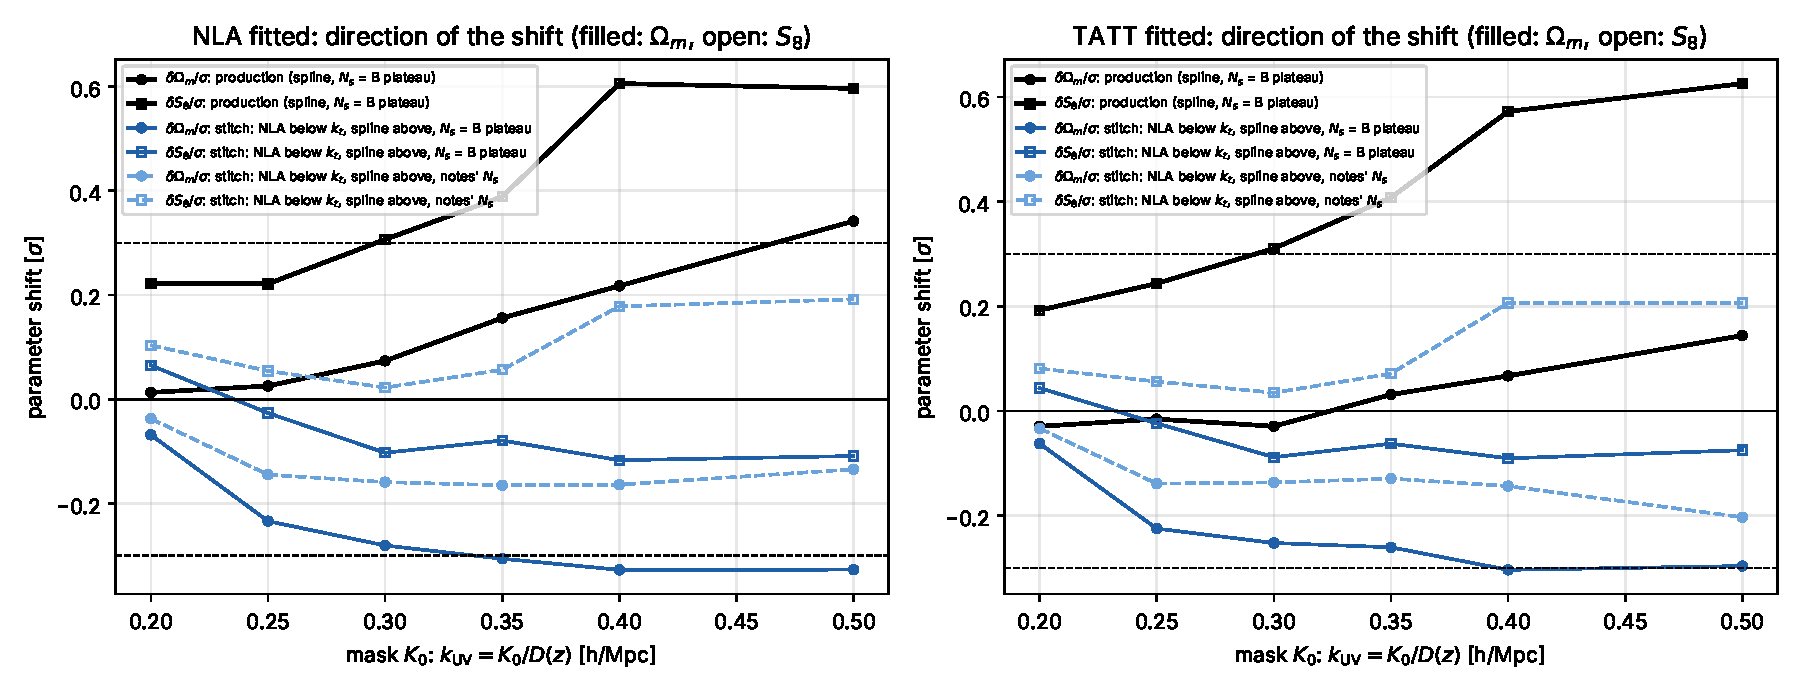
\includegraphics[width=\textwidth]{fig_stitch_shift}
\caption{The two components of the shift, $\delta\Omega_m/\sigma$ (filled)
and $\delta S_8/\sigma$ (open), against $K_0$ for the production truth and
the two stitched variants with the spline simulation side, case A. The
production shift is in $S_8$ and grows with $K_0$; the stitched shift is in
$\Omega_m$ and saturates.}
\end{figure}

\section{Reading the result}

\paragraph{Two failure modes.} The production FoB is the vector sum of two
things. (i) The white II excess $X(k) = (P_{EE} - N_s^{B}) - P_{\delta E}^2/P_{\rm NL}
\approx$ const, 1 to 2 times $N_s^B$, an E-mode white power 2 to 4 times the
B-mode white power. A white $P_{EE}$ gives a constant $C_\ell$, $\xi_+ = 0$
and $\xi_- = 2C/(\pi\theta^2)$, so it enters through the small-$\theta$
$\xi_-$ points that the $K_0$ masks release as $K_0$ grows; neither NLA nor
TATT has such a term, and both absorb it into $S_8$. This is the +0.3 to
+0.6$\sigma$ $S_8$ shift of the production truth and the reason its FoB
keeps growing with $K_0$. (ii) The misfit of the model GI and II shapes to
the simulation at $0.2 \lesssim k \lesssim 1\hmpc$ (the GI dip to 0.8 of
$C_1 P_{\rm NL}$ at $z \le 0.75$ and the II rise, Figure 1), which both
models absorb into $\Omega_m$ at the $-0.3\sigma$ level and which saturates
once the mask reaches $K_0 \approx 0.35$, because the $K_0/D$ masks add
little weight beyond that. The stitch removes (i) below $k_t$ (S1) or
everywhere (S2, S3; the notes' $N_s$ is 2.2 to 3.8 times the B plateau)
and leaves (ii) untouched, which is why $\chi^2$ barely moves while the
shift rotates from $S_8$ to $\Omega_m$.

\paragraph{Why S1 still reaches 0.3.} Below $k_t$ the S1 truth is NLA with
the notes' per-snapshot amplitude, which NLA with a free $(A_1, \eta_1)$
reproduces up to the mismatch between the per-snapshot amplitudes and a
single power law, and TATT nests NLA; the residual FoB of 0.12 / 0.10 at
$K_0 = 0.2$ is that mismatch plus the transition. From $K_0 = 0.25$ on the
masks reach past $k_t$ at $z \ge 0.5$ and the transition-regime misfit
takes over: $\delta\Omega_m = -0.23\sigma$ at 0.25, $-0.28\sigma$ at 0.3,
$-0.30\sigma$ at 0.35 (NLA), with $S_8$ within $\pm 0.1\sigma$. So even
granting the notes' NLA assumption on large scales, the cut cannot be
pushed past $K_0 \approx 0.35$ (NLA) or 0.4 (TATT) without a $0.3\sigma$
shift, now in $\Omega_m$.

\paragraph{Why it is not a conservative truth.} The v3 goodness of fit with
$N_s$ fixed rejects NLA at $k_{\max}$ = 0.09 to 0.12$\hmpc$ in every core
snapshot (combined $p = 10^{-7}$ at 0.12), and the measured ratios in
Figure 1 depart from the NLA plateau by 5 to 10 per cent between 0.1 and
$k_t$. The stitch asserts NLA there, with $w \le 0.5$, and that band
carries about 45 per cent of the Roman weight. The S1 minus production
$\dchi_{\rm Roman}$ of 2.3 to 4.8 (Table 1) is the size of the data-vector
change this assumption makes before any fit, comparable to the whole
residual $\chi^2$ of either model.

\paragraph{S2 and S3.} With the notes' $N_s$ the white term is gone at all
$k$ and the remaining difference from S1 is the over-subtraction above
$k_t$: FoB 0.17 / 0.15 at $K_0 = 0.3$ against 0.28 / 0.25 for S1, so the
white term that survives the S1 stitch above $k_t$ is worth about 0.1 in
FoB. S3 (measured instead of spline simulation side) differs from S2 by at
most 0.03 at $K_0 \le 0.4$: the FLAMINGO noise above $k_t$ is not what
drives any of this. At $K_0 = 0.5$ the TATT fits to S2 and S3 sit at the
$\eta_2$ and $b_{\rm TA}$ bounds.

\paragraph{Flat masks.} The $z$-dependent TATT-shaped cuts reach less far
in $k$ at high redshift than the $K_0/D$ family (at $z = 1$, 0.29 / 0.41 /
0.58$\hmpc$ for $f$ = 1 / 1.4 / 2, against 0.49 for $K_0 = 0.3$), so with the
large-scale term removed they keep every stitched FoB below 0.27, while the
production truth crosses 0.3 at $f \approx 1.3$ through the white term.

\paragraph{S4.} Replacing the held ratio below $k = 0.05$ by pure NLA
switches the white term off below the data $k_{\min}$ with a hard join;
$\dchi_{\rm Roman}$(S4 $-$ prod) is 1.1 to 1.6 and the fitted $\chi^2$
rises by 0.3 to 1.0 because neither model can follow the kink. The FoB
moves by at most 0.05 (NLA) and +0.03 to +0.08 (TATT, now at the $\eta_2$
bound). The smooth alternative, white term held white below 0.05
(\texttt{bias\_phys.py}: FoB 0.22 / 0.24, 0.40 / 0.41, 0.64 / 0.63 at
$K_0$ = 0.25, 0.35, 0.5), changes the production FoB by less than 0.02 and
is the extrapolation to quote.

\paragraph{Case B.} For S1 on the $K_0/D$ masks, freeing $n_s$, $H_0$,
$\Omega_b$ with the chain priors changes the FoB by $-0.01$ to $+0.06$
(largest for TATT at $K_0 \ge 0.35$), as for the production truth.

\section{Code}
\begin{itemize}\sloppy
\item \texttt{v3/stitched\_test.py}: builds the five truths (ratios on the
  data grid, \texttt{stitched\_truths.npz}), the sim\_IA tables and $\xi$
  vectors (\texttt{stitched\_xi.npz}), runs the fits
  (\texttt{roman\_test.fit}) on every mask and writes
  \texttt{stitched\_test.json}, \texttt{stitched\_test\_log.txt}.
\item \texttt{v3/plot\_stitched.py}: \texttt{fig\_stitch\_truths},
  \texttt{fig\_stitch\_fob}, \texttt{stitched\_test.csv}.
\item Inputs: \texttt{v2/fits.npz} (spline truth, data, errors, $N_s^{B}$),
  \texttt{spectra.npz} (notes' stitch: $C_1$, $N_s^{\rm NLA}$,
  \texttt{truth\_nla}; from \texttt{build\_spectra.py}),
  \texttt{tatt\_fit/fit\_stitched\_kmax.py} ($k_t$, $w$),
  \texttt{v3/masks\_v3.npz}, \texttt{cocoa/run/cosmolike\_xi\_ia.npz},
  \texttt{cocoa/analysis/cov\_gauss\_d3a.npy}, \texttt{cocoa/analysis/J\_cells.npy};
  \texttt{v3/roman\_test.py} and \texttt{cocoa/bias\_v2.py} for the fit.
\end{itemize}
\end{document}
